\documentclass[t]{beamer}

\usepackage[english]{babel}
\usepackage[utf8]{inputenc}
\usepackage[T1]{fontenc}

\usepackage{amsmath}
\usepackage{amssymb}
\usepackage{float}
\usepackage{graphicx}
\graphicspath{{../images/}}
\usepackage{tikz}
\usepackage{hyperref}
\hypersetup{
    colorlinks,
    citecolor=black,
    filecolor=black,
    linkcolor=black,
    urlcolor=blue
}
\usepackage{array}
\usepackage{booktabs}

\usetheme{metropolis}

\usepackage{lmodern}
\usepackage[scale=2]{ccicons}

\title{Data-driven Confocal Microscopy to Hematoxylin and Eosin Transformation}
\subtitle{Digitally Stained Confocal Microscopy through Deep Learning}
\author{Sergio García Campderrich}
%\institute{Universitat Politècnica de Catalunya}
\date{\today}

%% Custom commands
\newcommand{\cycleGAN}[2]{G_{#1 \rightarrow #2}}
\newcommand{\tensor}[1]{\mathbf{#1}}
\newcommand{\R}{\mathbb{R}}
\DeclareMathOperator*{\argmax}{arg\!\max}
\DeclareMathOperator*{\argmin}{arg\!\min}

\begin{document}
\setbeamertemplate{caption}{\raggedright\insertcaption\par}
\maketitle

\begin{frame}
\frametitle{Contents}

\begin{itemize}
\item Introduction\pause
\item Theoric background\pause
\item Methodology\pause
\item Experiments and results\pause
\item Conclusions and future development
\end{itemize}

\end{frame}


\AtBeginSubsection[]
  {
     \begin{frame}<beamer>
     \tableofcontents[currentsubsection,sections=\thesection]
     \end{frame}
  }

\section{Introduction}

\subsection{Hematoxylin and Eosin (H\&E)}

\begin{frame}
\frametitle{What is it?}

\begin{columns}

\begin{column}{0.5\textwidth}
\begin{figure}
\centering
\only<1->{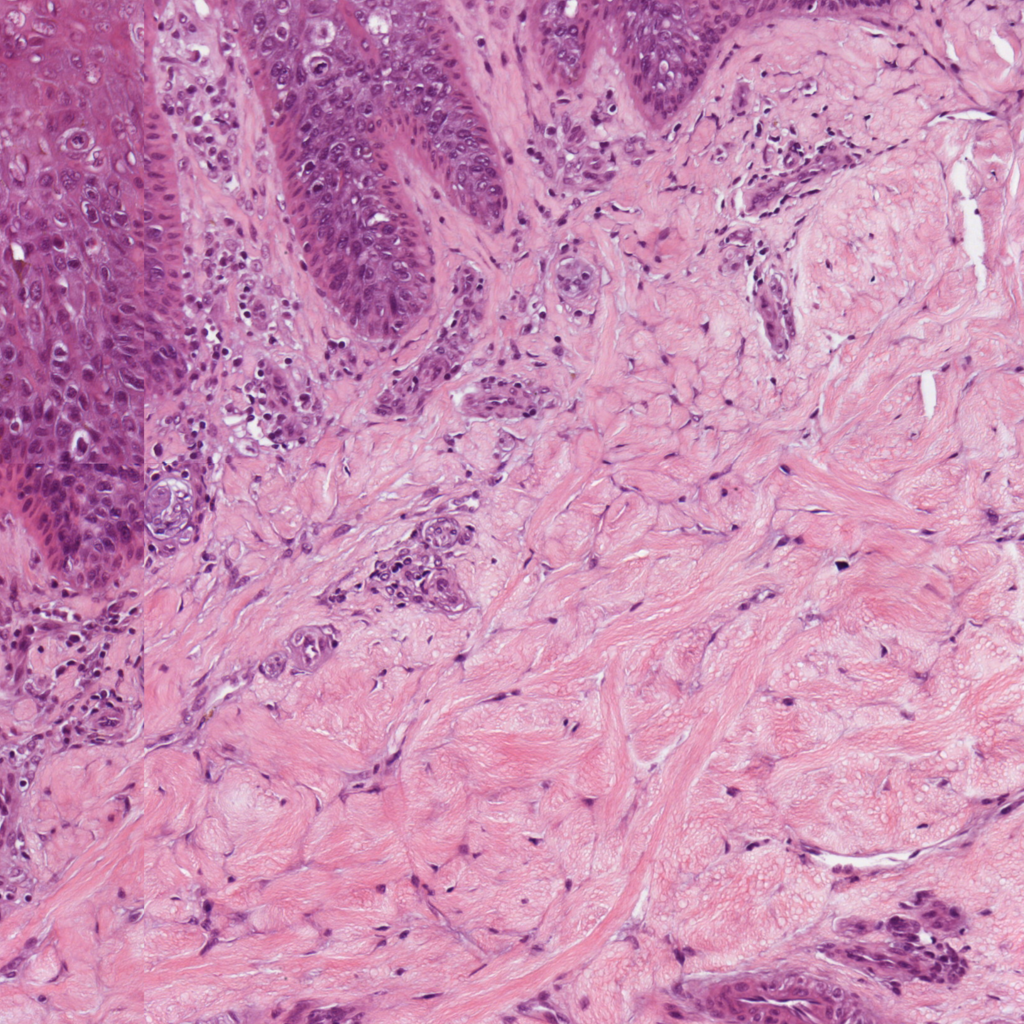
\includegraphics[width=0.9\textwidth]{HE-2}
\caption{H\&E stained tissue sample}}
\end{figure}
\end{column}\pause

\begin{column}{0.5\textwidth}
\only<2-3>{
\begin{block}{Usage}
\begin{itemize}
\item<2-3> Hematoxylin and eosin stain (H\&E stain) is one of the principal tissue stains used in histology and Mohs sugery.
\item<3> The \textbf{hematoxylin} stains cell nuclei \textbf{blue}, and \textbf{eosin} stains the
extracellular matrix and cytoplasm \textbf{pink}, with other structures taking on different shades, hues,
and combinations of these colors.
\end{itemize}
\end{block}
}
\only<4->{
\begin{alertblock}{It can be a slow process}
\begin{itemize}
\item<4-5> Tissues are typically frozen, cut, fixed in alcohol and then stained.
\item<5> Involves application of hematoxylin mixed with a metallic salt, a rinse in a weak acid solution, followed by bluing in alkaline water.
After the application of hematoxylin, the tissue is counterstained with eosin.
\end{itemize}
\end{alertblock}
}
\end{column}

\end{columns}
% La histología es la rama de la biología que estudia la composición, la estructura y las características de los tejidos orgánicos de los seres vivos.

% La cirugía de Mohs, es un tipo de cirugía microscópica controlada, altamente eficaz para tratar ciertos tipos comunes de cáncer de piel.
% controla micrográficamente, de manera que el paciente permanece en el quirófano mientras se estudia por microscopio el tejido extraído, proporciona el retiro exacto del tejido canceroso, mientras que se ahorra el tejido sano.
\end{frame}

\subsection{Confocal microscopy}

% La microscopía confocal es una tecnología que permite a los patólogos el análisis rápido de muestras de tejido para la detección de carcinomas.
% Sin embargo, esta tecnología aún no se ha establecido en la práctica clínica estándar porque la mayoría de los patólogos carecen del conocimiento para interpretar su salida.

\begin{frame}
\frametitle{What is it?}

CM is an optical imaging technique for increasing optical resolution and contrast of a micrograph
by means of using a spatial pinhole to block out-of-focus light in image formation.

It is able to capture multiple two-dimensional images at different depths in a sample (a process known as optical sectioning).

\begin{figure}
\centering
     \only<1>{
     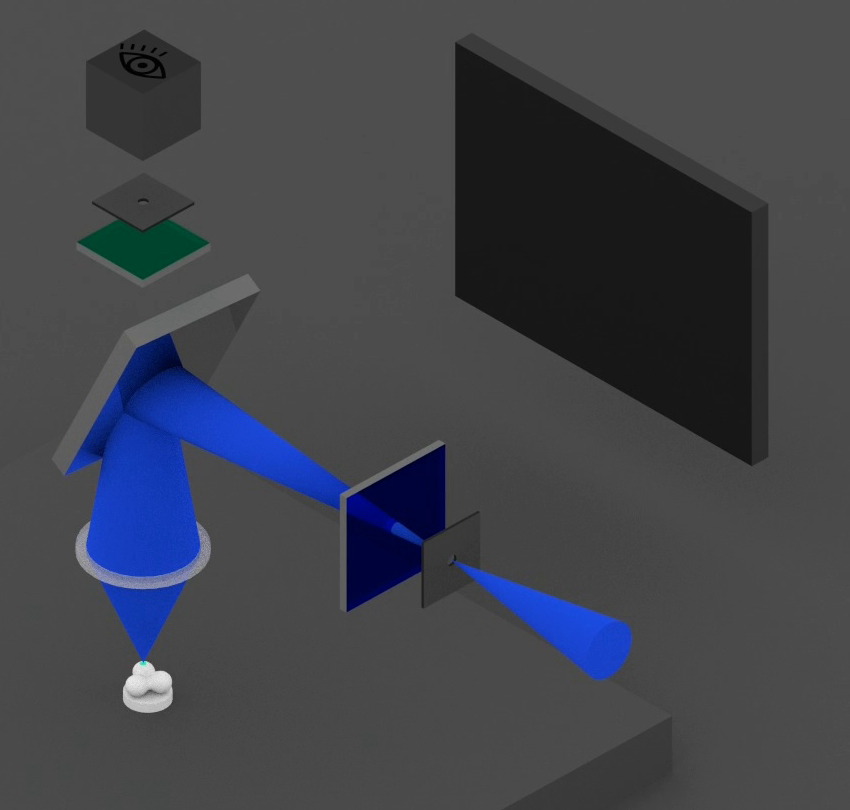
\includegraphics[scale=0.1]{CM-process-1-1}\hspace{0.1\textwidth}%
     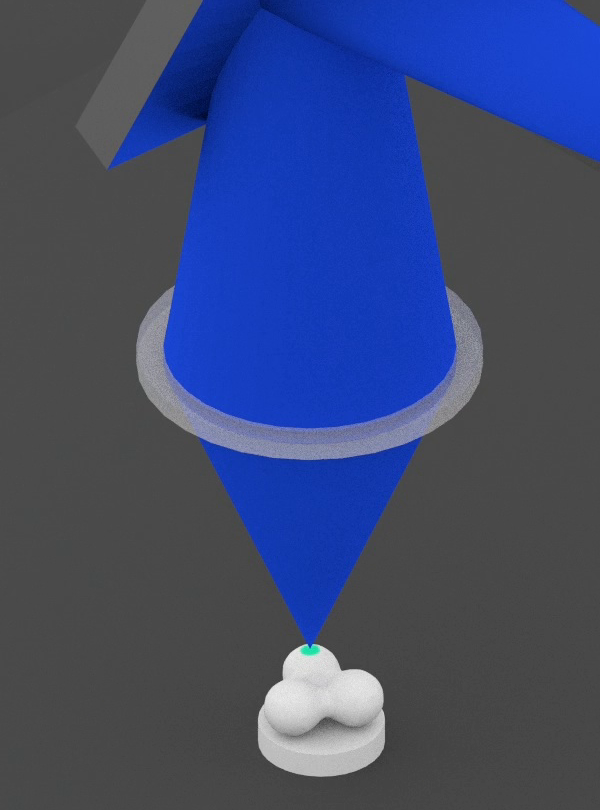
\includegraphics[scale=0.1]{CM-process-1-2}
     \caption{\footnotemark{}The light beam is focused by a pinhole on a small part of the sample}
     }
     \only<2>{
     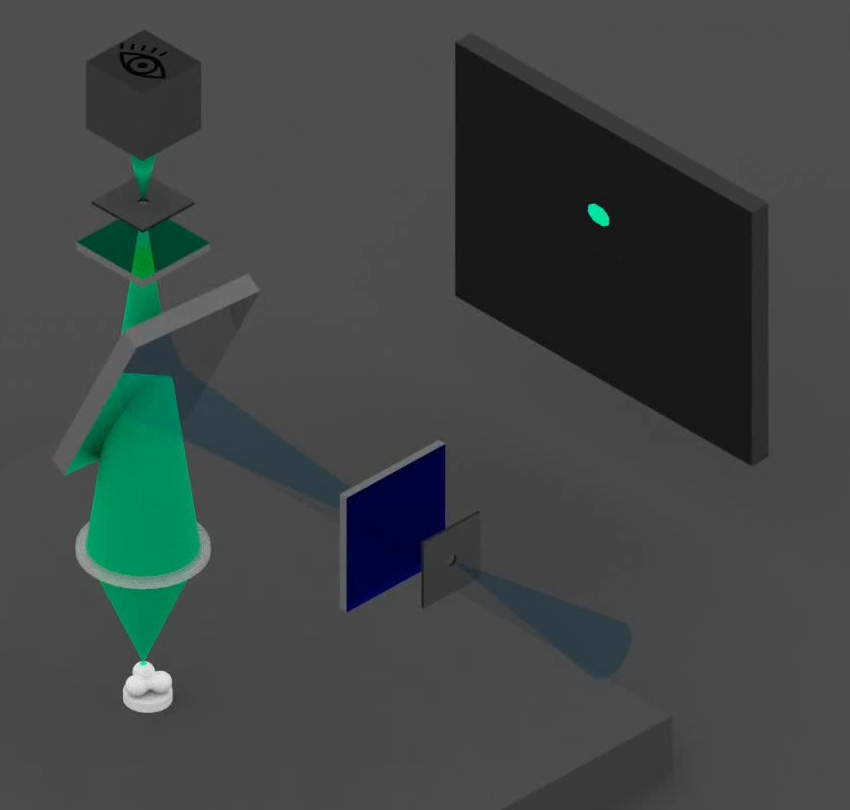
\includegraphics[scale=0.1]{CM-process-2-1}\hspace{0.1\textwidth}%
     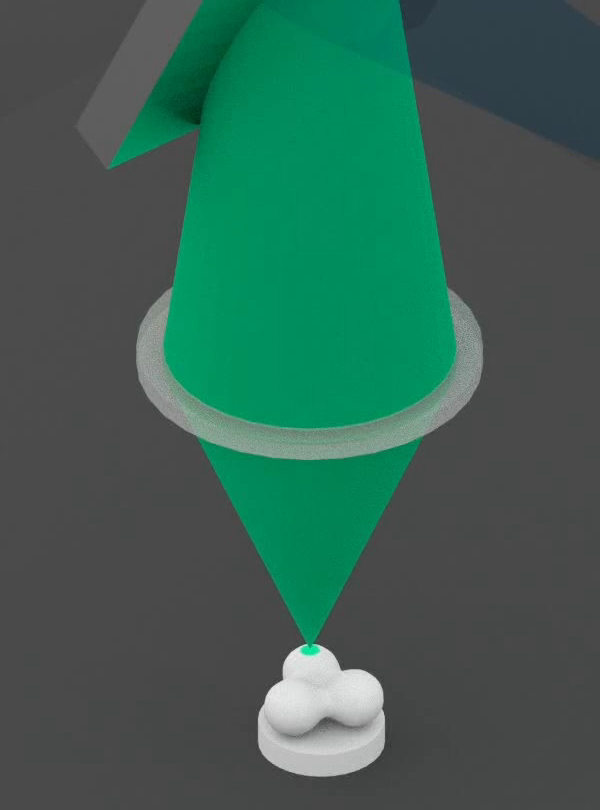
\includegraphics[scale=0.1]{CM-process-2-2}
     \caption{\footnotemark{}If fluorosphores are present, they emit light}
     }
     \only<3>{
     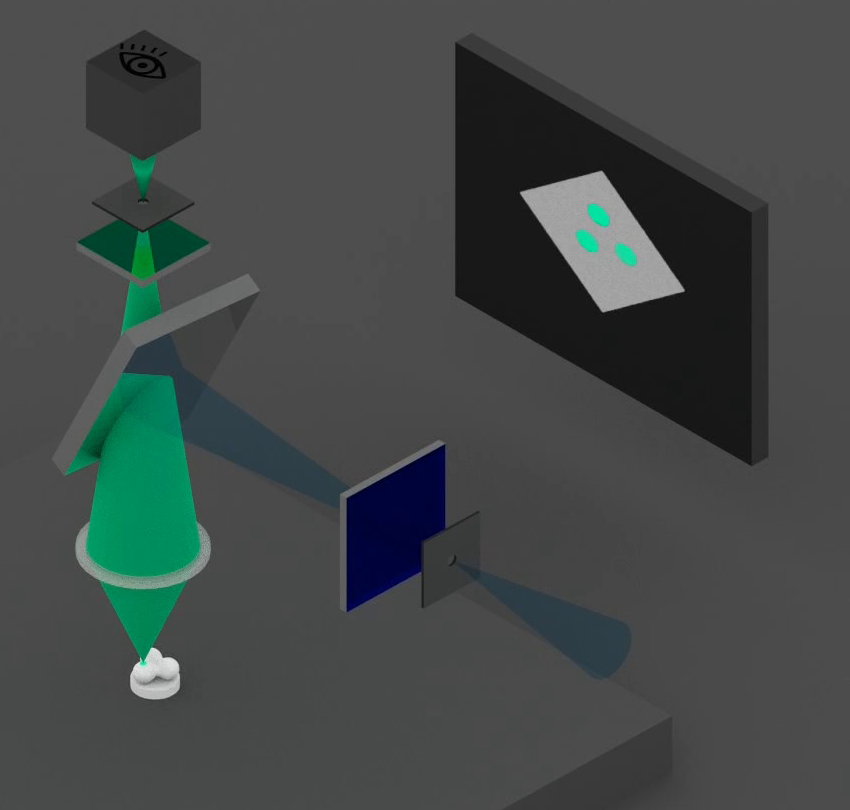
\includegraphics[scale=0.1]{CM-process-3-1}\hspace{0.1\textwidth}%
     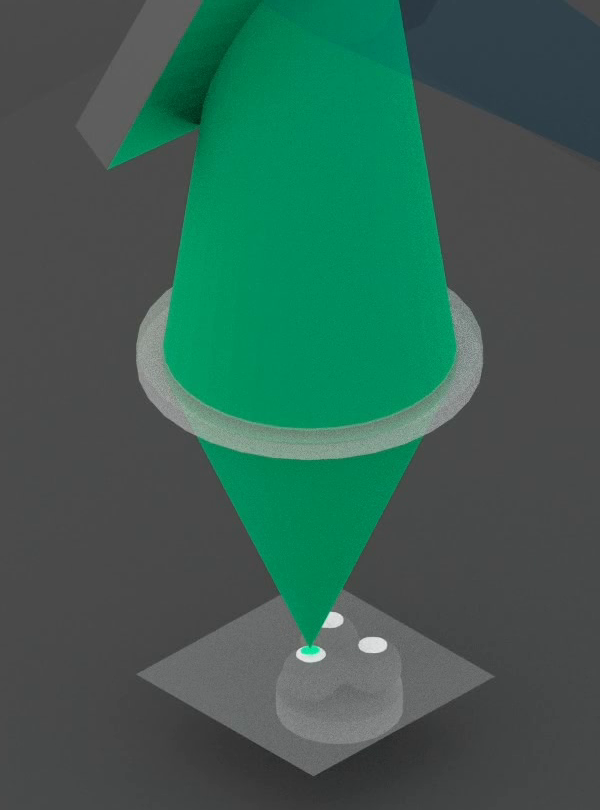
\includegraphics[scale=0.1]{CM-process-3-2}
     \caption{\footnotemark{}The surface is scanned by moving the sample/light beam}
     }
     \only<4>{
     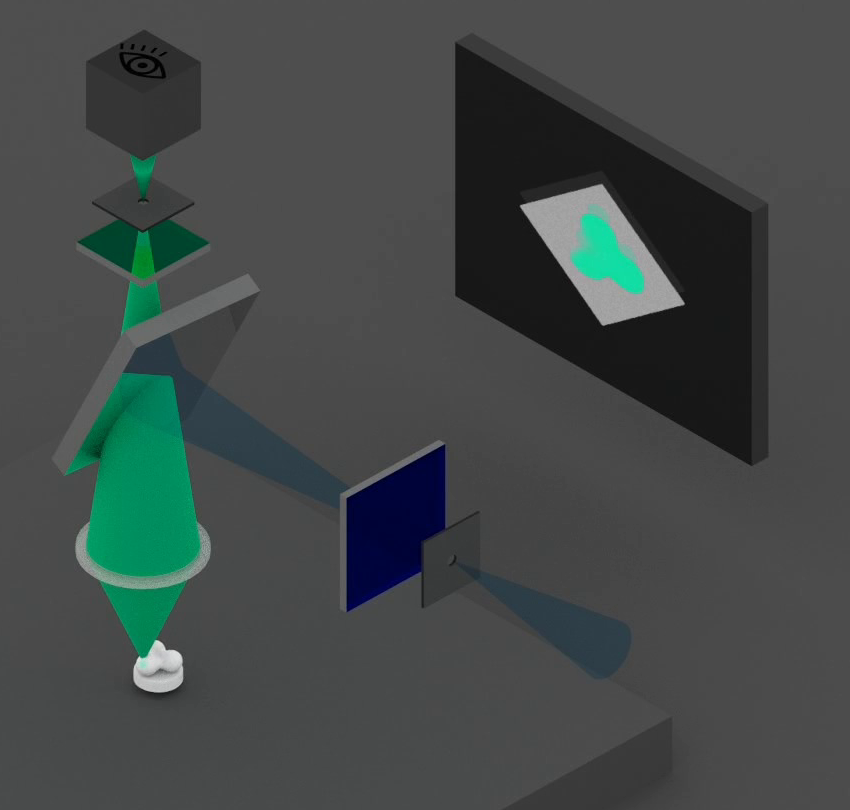
\includegraphics[scale=0.1]{CM-process-4-1}\hspace{0.1\textwidth}%
     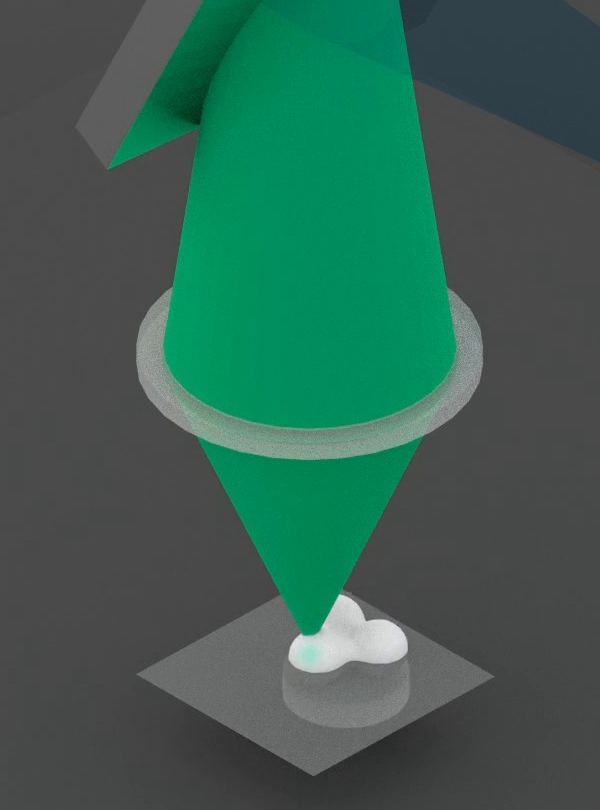
\includegraphics[scale=0.1]{CM-process-4-2}
     \caption{\footnotemark{}One can move vertically to obtain images at different heights}
     }
\end{figure}

\only<2->{
	\footnotetext{Images extracted from \href{https://commons.wikimedia.org/wiki/File:Fluorescent_and_confocal_microscopes.ogv}{wikimedia}.}
}

\end{frame}

\begin{frame}{Similarities and dissimilarities with H\&E}
    \begin{block}{Similarities}<1->
    {
        \begin{itemize}
        \item Usage in histopathology
        \item Up to cellular level resolution
	\item Expose similar structures in tissues
        \end{itemize}
    }
    \end{block}
    \begin{alertblock}{Differences}<2>
    {
        \begin{itemize}
        \item Specimens can be examined in near real-time without time consuming processing procedures.
        \item Output largely diers from the standard H\&E slides
        \end{itemize}
    }
    \end{alertblock}

\end{frame}

\begin{frame}{Modes}

In addition to ``standard'' reflection mode, CM can work in fluorescent mode for specimens stained with fluorochromes.

\only<1>{
\begin{columns}

\begin{column}{0.5\textwidth}
\begin{figure}
\centering
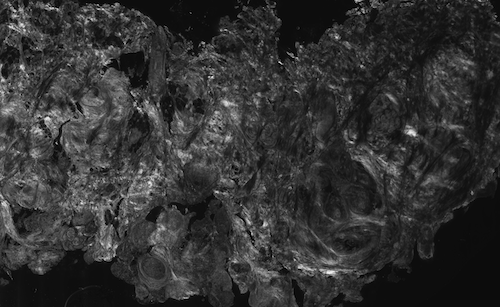
\includegraphics[width=0.9\textwidth]{CM-R}
\caption{Reflectance mode}
\end{figure}
\end{column}

\begin{column}{0.5\textwidth}
\begin{figure}
\centering
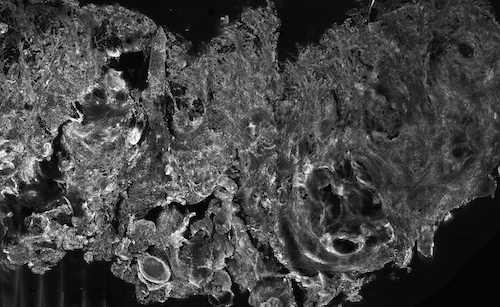
\includegraphics[width=0.9\textwidth]{CM-F}
\caption{Fluorescence mode}
\end{figure}
\end{column}
\end{columns}
}

\only<2>{
\begin{columns}

\begin{column}{0.5\textwidth}
\begin{figure}
\centering
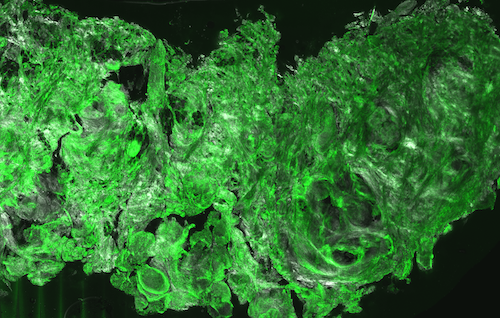
\includegraphics[width=0.9\textwidth]{CM-blend}
\caption{Blend of reflectance and fluorescence mode.}
\end{figure}
\end{column}

\begin{column}{0.5\textwidth}
\begin{figure}
\centering
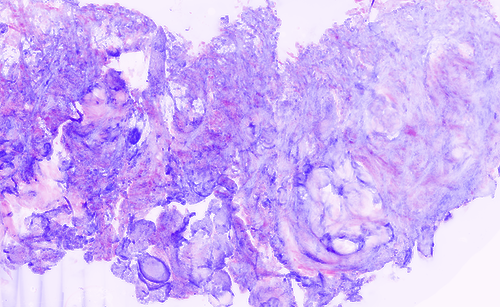
\includegraphics[width=0.9\textwidth]{CM-pseudocolor}
\caption{Pseudocolor/falsecolor H\&E-like digital stain from reflectance and fluorescence modes}
\end{figure}
\end{column}
\end{columns}
}


\end{frame}

\subsection{Data-driven transformation}

% Para abordar este problema, se presenta y evalúa un método basado en datos para transformar las micrografías confocales en imágenes parecidas a hematoxilina y eosina de aspecto más familiar, lo que permite a los patólogos interpretar estas imágenes sin formación específica.

\begin{frame}{Why?}
As confocal micrographs largely differ from the standard H\&E slides that
pathologists typically use to analyze tissue samples, professionals need
to undergo specific training.

A correctly done CM to H\&E mapping should bring the efficiency of CM
to untrained pathologists and surgeons.

\begin{columns}

\begin{column}{0.5\textwidth}
\begin{figure}
\centering
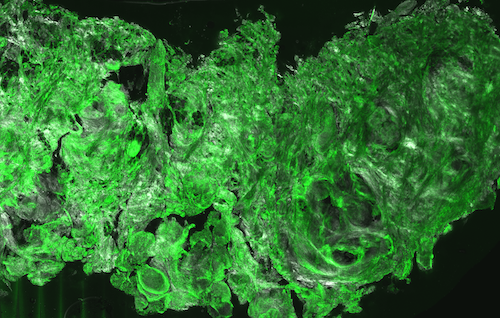
\includegraphics[width=0.9\textwidth]{CM-blend}
\end{figure}
\end{column}

\begin{column}{0.5\textwidth}
\begin{figure}
\centering
\includegraphics[scale=0.6]{doctor}
\end{figure}
\end{column}

\end{columns}
\end{frame}

\begin{frame}{Why?}
Standard pseudocolor transformation is a linear transformation that cannot capture the true appearance of H\&E stained samples.

Different structures should be mapped to different colours even if the pixel values are the same.

\begin{columns}

\begin{column}{0.5\textwidth}
\begin{figure}
\centering
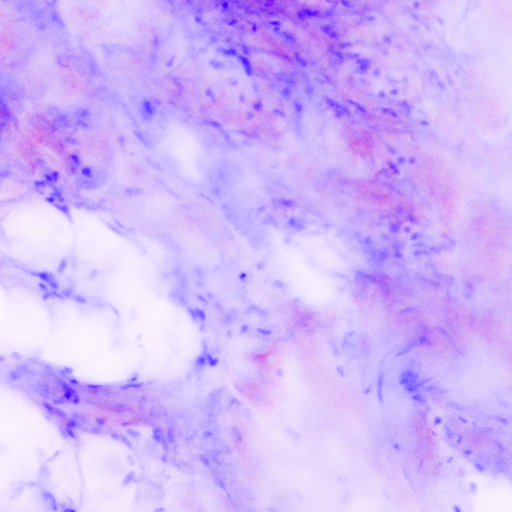
\includegraphics[width=0.5\textwidth]{epoch246_real_A}
\caption{Colors and structures greatly vary from the ones found in H\&E slides}
\end{figure}
\end{column}

\begin{column}{0.5\textwidth}
\begin{figure}
\centering
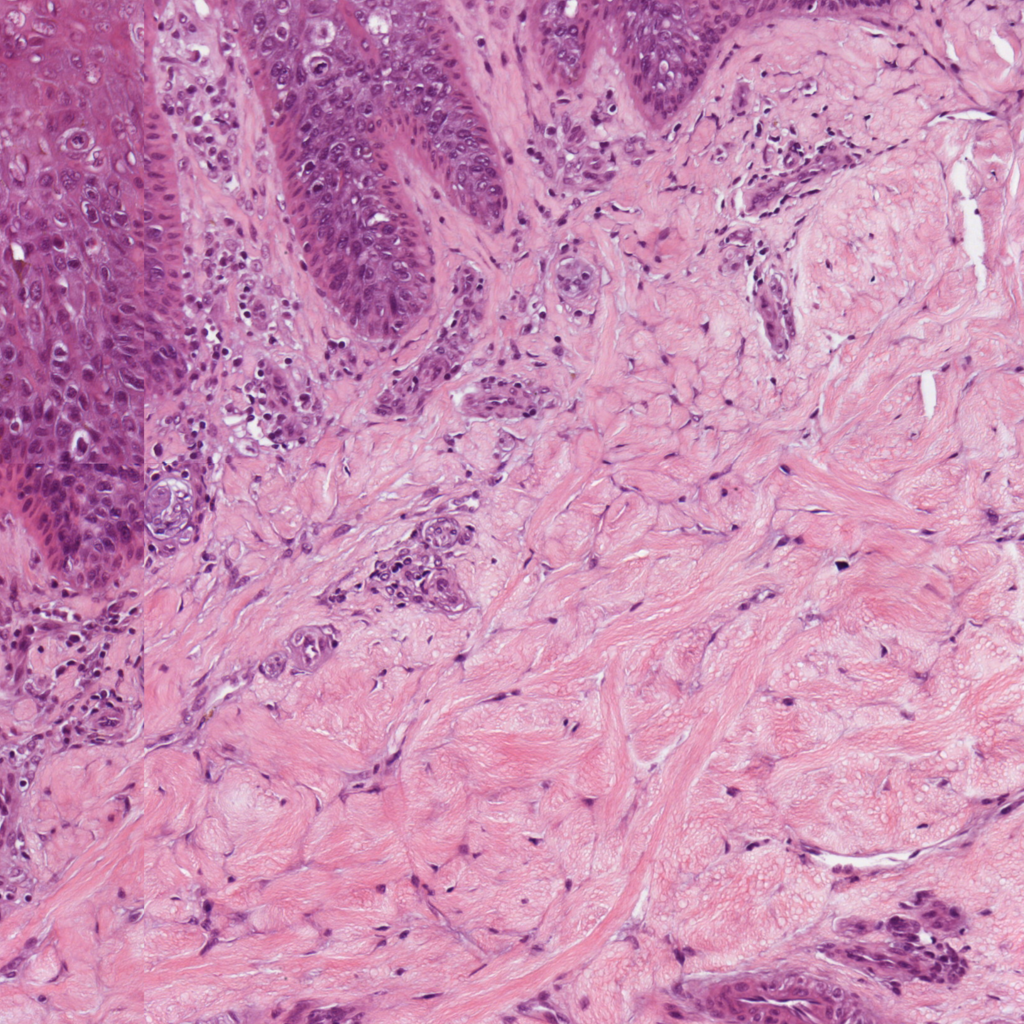
\includegraphics[width=0.5\textwidth]{HE-2}
\caption{H\&E slide}
\end{figure}
\end{column}

\end{columns}

\end{frame}

\begin{frame}{How?}
% El principal obstáculo para definir dicha transformación es la ausencia de datos confocales emparejados con imágenes de hematoxilina y eosina que necesitan los marcos tradicionales de aprendizaje automático. Para superar este problema, se utiliza el marco de redes generativas antagónicas de ciclo consistente.
% Este marco presenta problemas específicos como el entrenamiento inestable y la ``alucinación'' o eliminación de estructuras que este trabajo intenta cuantificar y mitigar.

\begin{figure}
\centering
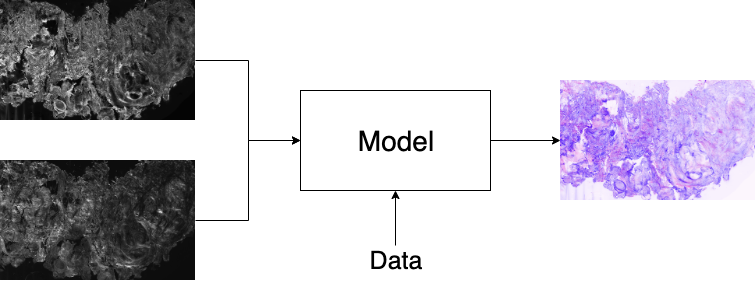
\includegraphics[width=0.5\textwidth]{transformation}
\end{figure}

\begin{columns}

\begin{column}{0.6\textwidth}
\only<2->{
\begin{block}{Solution}
\begin{itemize}
\item<2-> Data driven approach to try to find a better transformation
\item<3-> CNNs are good at \emph{learning} non-linear mappings
\item<5-> Use CycleGANs framework
\end{itemize}
\end{block}
}
\end{column}

\begin{column}{0.4\textwidth}
\only<4->{
\begin{alertblock}{But}
\begin{itemize}
\item Traditional solutions require pairs of CM and H\&E slides, which would be very difficult
\end{itemize}
\end{alertblock}
}
\end{column}

\end{columns}

\end{frame}


\section{Theoric background}

\subsection{Artificial neural networks}

\begin{frame}{Convolutional neural networks (CNNs)}

\begin{columns}

\begin{column}{0.4\textwidth}
\begin{tikzpicture}[baseline=(current bounding box.north)]
  \node (img1) {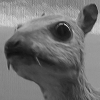
\includegraphics[width=0.3\textwidth]{conv-orig}};
  \onslide<2->{\node (img2) at (img1.north east) [xshift=0.25\textwidth] {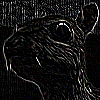
\includegraphics[width=0.3\textwidth]{conv-edge}};}
  \onslide<3->{\node (img3) at (img2.south east) {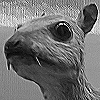
\includegraphics[width=0.3\textwidth]{conv-sharp}};}
  \onslide<4->{\node (img4) at (img3.south east) {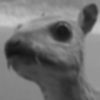
\includegraphics[width=0.3\textwidth]{conv-blur}};}
\end{tikzpicture}
\end{column}

\begin{column}{0.6\textwidth}
\begin{figure}
\onslide<5->{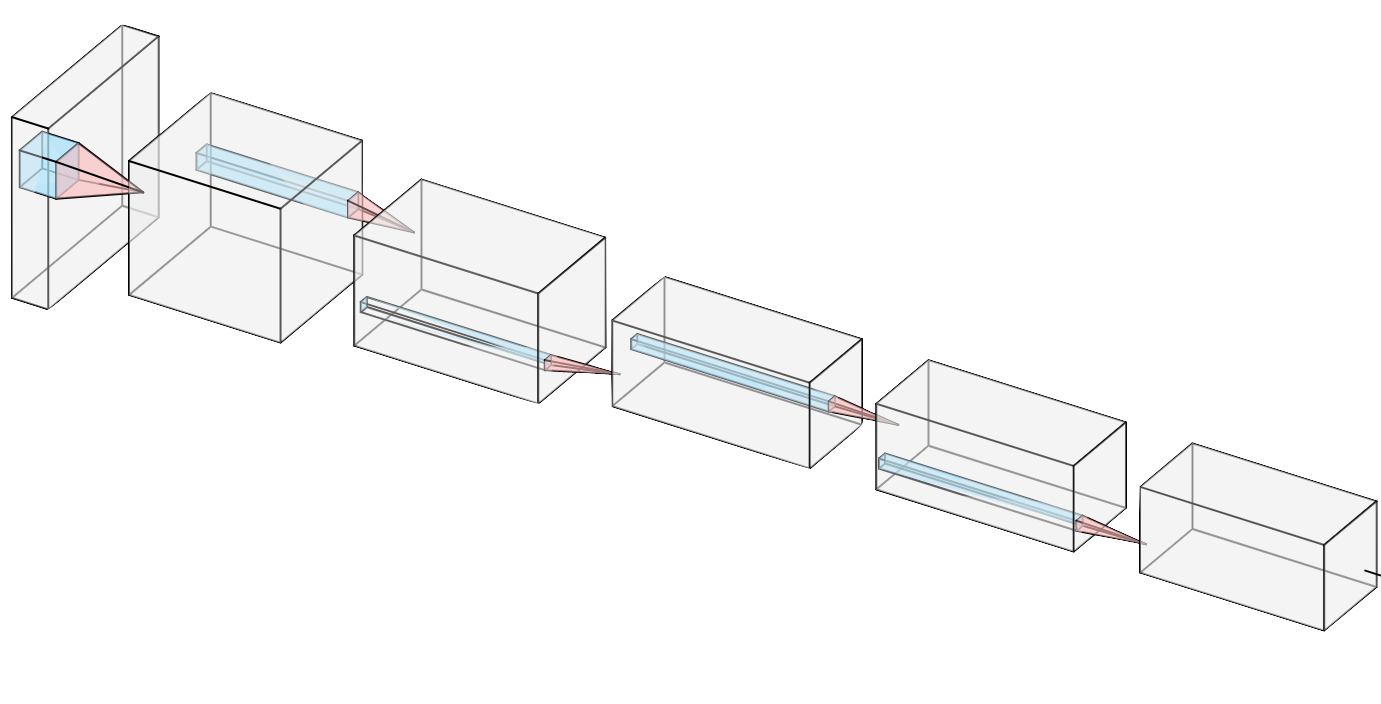
\includegraphics[width=0.8\textwidth]{fcnn}}
\end{figure}
\end{column}

\end{columns}

\begin{block}{Short description}
\begin{itemize}
\item Convolution is fast way to apply a linear translation-invariant transformation
\item<5-> A layer contains multiple filters
\item<5-> A layer's output is the concatenation of each resulting convolution
\end{itemize}
\end{block}

\end{frame}

\begin{frame}{Training}
% Differentiable by construction.
% Define an objective function a use gradient descent.
% Mention backpropagation algorithm.
% Defining an objective function for our problem is difficult (unpaired data)

\begin{block}{Define an objective function and optimize it}
\[
\theta^* = \argmin_{\theta} \mathcal{J}
\left( (\tensor{X}, \tensor{Y}), f_{\theta} \right)
\]

Neural networks are fully differentiable by construction, so we can use gradient-based methods.
\end{block}\pause

\begin{alertblock}{But}
Defining an objective function for our problem is straightforward.

We want to \emph{generate} images that \emph{look like} H\&E and are \emph{realistic}.
\end{alertblock}

\end{frame}

\subsection{Generative models}

\begin{frame}
\frametitle{Generative adversarial networks (GANs)}
% Quick and simple visual explanation.
Framework for estimating generative models via an adversarial
process, in which two models are trained: a generative model $G$ that captures
the data distribution, and a discriminative model $D$.

\begin{block}{Two-player minimax game}
\[
\min_G \max_D \mathbb{E}_{x \sim p_{data}(x)}\{\log D(x)\} +
\mathbb{E}_{z \sim p_z(z)} \{\log(1 - D(G(z)))\}
\]
\end{block}\pause

\begin{block}{Intuitively}
Two models ``fight'' one against the other (over the discriminator's loss)
in such a way that they improve each other, until the generator's samples are
indistiguishable from data.
\end{block}

\end{frame}

\begin{frame}[b]
\frametitle{Visual representation}
\begin{figure}
     \only<1>{
     
\includegraphics[scale=0.4]{GANs_animation-1}
     \caption{Discriminator predicts the probability of being ``real'' of a sample drawn from the dataset}
     }
     \only<2>{
     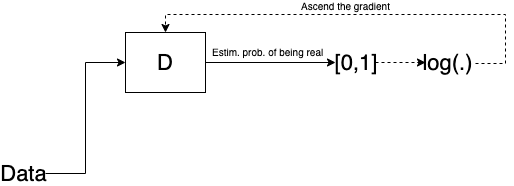
\includegraphics[scale=0.4]{GANs_animation-2}
     \caption{The discriminator's parameters are updated to increase the log-likelihood}
     }
     \only<3>{
     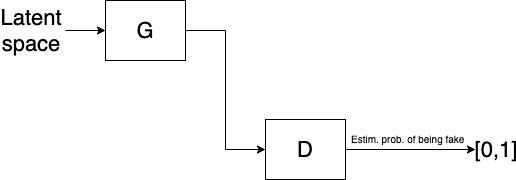
\includegraphics[scale=0.4]{GANs_animation-3}
     \caption{Discriminator predicts the probability of being ``fake'' of a sample drawn from the generator}
     }
     \only<4>{
     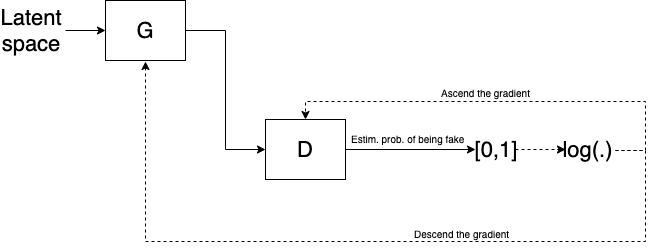
\includegraphics[scale=0.4]{GANs_animation-4}
     \caption{The discriminator's parameters are updated to increase the log-likelihood.
     The generator's parameters are updated to decrese the log-likelihood of the discriminator}
     }
\end{figure}

\end{frame}

\begin{frame}{Cicle-consistent GANs (CycleGANs)}
% Quick and simple visual explanation.
\only<1->{\begin{block}{Objective}
\begin{itemize}
\item Framework for image-to-image translation based on GANs, where
mapping is learned with unpaired data\pause

\item Unpaired data consists of a source set $\tensor{X}$ and a target set $\tensor{Y}$
with no information provided as to which $\tensor{x}_i$ matches which $\tensor{y}_i$
\end{itemize}
\end{block}
}

\only<2>{\begin{figure}
     \centering
     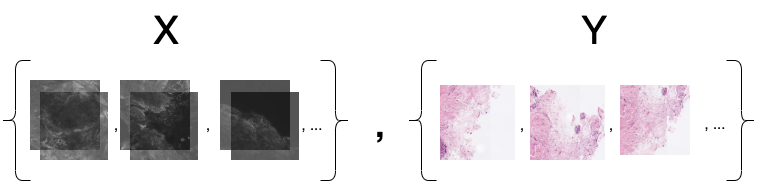
\includegraphics[scale=0.4]{unpaired_data}
\end{figure}
}
\only<3->{
\begin{alertblock}{Why not ``simple'' GANs?}
\begin{itemize}
\item<3-> Simply using the discriminator loss is not sufficient as it leads to the problem known as mode-collapse
where the generator ignores the source

\item<4-> This problem is addressed by ``encouraging'' the mapping to be cycle-consistent, i.e.:
$ \cycleGAN{Y}{X}(\cycleGAN{X}{Y}(\tensor{x})) \approx \tensor{x} $.
\end{itemize}
\end{alertblock}
}

\end{frame}

\begin{frame}{Cycle-consistent GANs (CycleGANs)}

\only<1->{
\begin{block}{Two pairs of generator-discriminator are trained}
\begin{itemize}
\item $\cycleGAN{X}{Y}$ maps from domain $X$ to domain $Y$. $D_Y$ discriminates in domain $Y$.
\item $\cycleGAN{Y}{X}$ maps from domain $Y$ to domain $X$. $D_X$ discriminates in domain $X$.
\end{itemize}
\end{block}
}

\only<2->{
\begin{columns}

\begin{column}{0.4\textwidth}
\begin{figure}
\centering
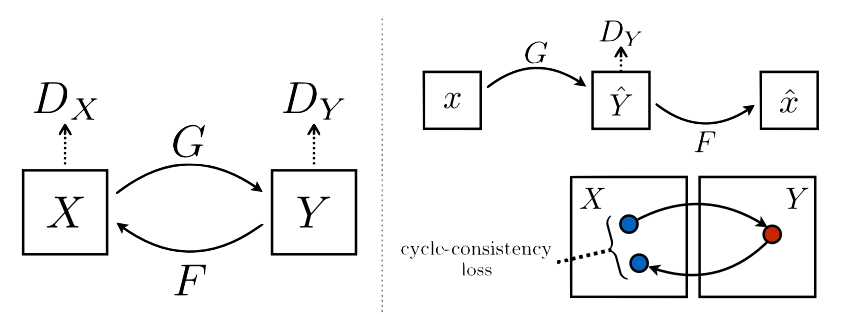
\includegraphics[width=\textwidth]{cyclegan-diagram-small}
\end{figure}
\end{column}

\begin{column}{0.6\textwidth}
Modified loss for $\cycleGAN{X}{Y}$ (analogous for $\cycleGAN{Y}{X}$):
\[
\begin{split}
\mathcal{L}_{\cycleGAN{X}{Y}} = &\log(1 - D_Y(\cycleGAN{X}{Y}(\tensor{x}))) \\
&+ \lambda \left\| \tensor{x} -
\cycleGAN{Y}{X}(\cycleGAN{X}{Y}(\tensor{x})) \right\|_1 \\
\end{split}
\]
\end{column}

\end{columns}
}

\end{frame}


\section{Methodology}

\subsection{Despeckling}

\begin{frame}{Speckle noise}
% Que es?
% Modelo de ruido
% Ejemplo del dataset
The reflectance CM image is corrupted by speckle:\\
Scattered signals add constructively and destructively depending on the relative phases of each scattered waveform.
Speckle results from these patterns of constructive and destructive interference shown as bright and dark dots in the image.

\begin{columns}

\begin{column}{0.5\textwidth}
\begin{figure}
\centering
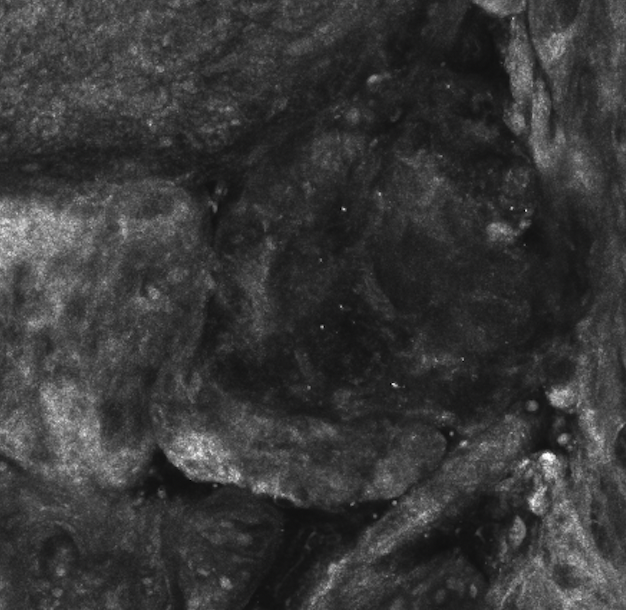
\includegraphics[width=0.5\textwidth]{speckle-1}
\caption{Example of speckled RCM image}
\end{figure}
\end{column}

\begin{column}{0.5\textwidth}
\only<2->{
\begin{block}{Speckle model}
\[ Y = X \odot F \]
\[ F \sim \Gamma(k = L, \theta = \frac{1}{L}) \]
\end{block}
}
\end{column}

\end{columns}

\end{frame}

\begin{frame}{Despeckling network}
A CNN is used to filter speckle noise prior to the stain transformation.\pause

\begin{figure}
\centering
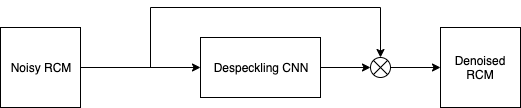
\includegraphics[scale=0.3]{despeckling-nn_multiplicative}
\caption{Model with multiplicative skip-connection}
\end{figure}\pause

\begin{figure}
\centering
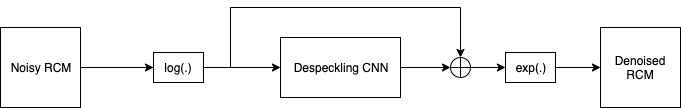
\includegraphics[scale=0.3]{despeckling-nn_additive}
\caption{Model with additive skip-connection}
\end{figure}

\end{frame}

\begin{frame}{Training}

\begin{block}{Loss}
The models are trained using the MSE loss:
\[ \mathcal{L} = \left\| \tensor{x}_{clean} - f_{\theta}(\tensor{x}_{noisy}) \right\|_2 \]
\end{block}\pause

\begin{block}{Data}
Due to the impossibility to obtain the noisy and clean versions of the the RCM images,
artificially contaminated FCM images are used to obtain the ($\tensor{x}_{clean}$, $\tensor{x}_{noisy}$) pairs.
\end{block}
\begin{figure}
\centering
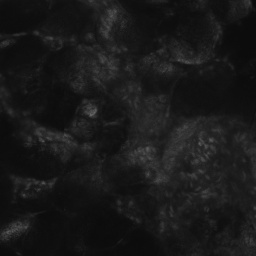
\includegraphics[width=0.2\textwidth]{9_768-6912_F-thumbnail}\hspace{0.15\textwidth}%
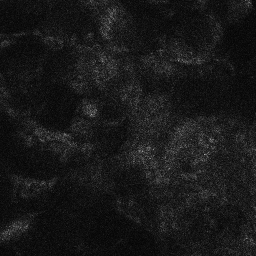
\includegraphics[width=0.2\textwidth]{9_768-6912_F-thumbnail_noisy}
\end{figure}

\end{frame}

\subsection{Stain}

\begin{frame}{Generators' architecture}
Both families follow an encoder-decoder
structure, i.e.: a series of convolution layers with down-sampling (encoder)
followed by the same number of layers with up-sampling\footnotemark{} (decoder),
presumably the encoder maps the input into a latent representation where
semantic transformations can be more easily defined and then the decoder
``brings'' it back to the image space.

\begin{figure}
\centering

\includegraphics[width=0.6\textwidth]{encoder-decoder}
\caption{\href{https://arxiv.org/abs/1511.00561}{image credits}}
\end{figure}

\end{frame}

\begin{frame}{Residual network}

\begin{figure}
\centering
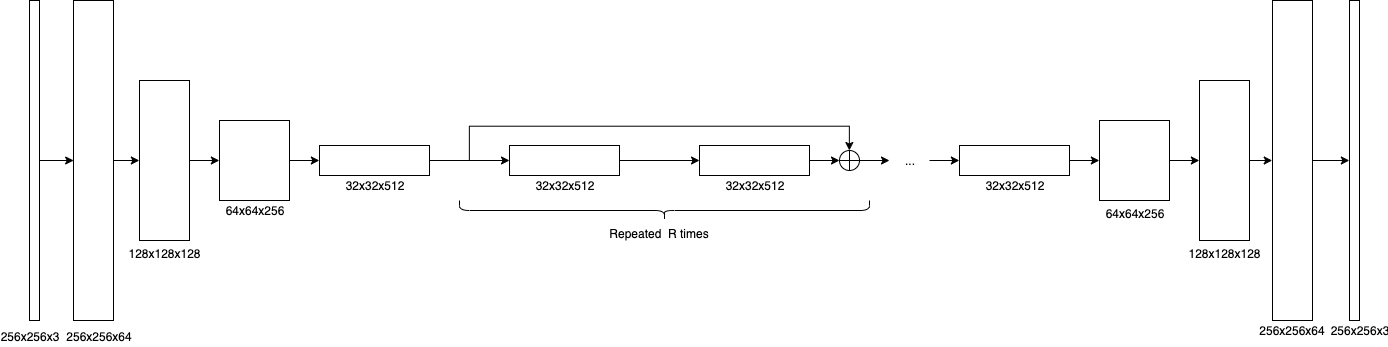
\includegraphics[width=0.9\textwidth]{residual_stain-nn}
\end{figure}

In a residual block, intead of trying to learn
a transformation $\mathcal{T}(\tensor{x})$, the residual
$\mathcal{F}(\tensor{x})$ is learnt so that
$\mathcal{T}(\tensor{x}) = \mathcal{F}(\tensor{x}) + \tensor{x}$
the motivation behind this is to
avoid the problem know as the degradation problem where deeper networks
perform worse than shallower counterparts, when in theory they should at
least perfom equally well.

\end{frame}

\begin{frame}{UNet-like network}

\begin{figure}
\centering
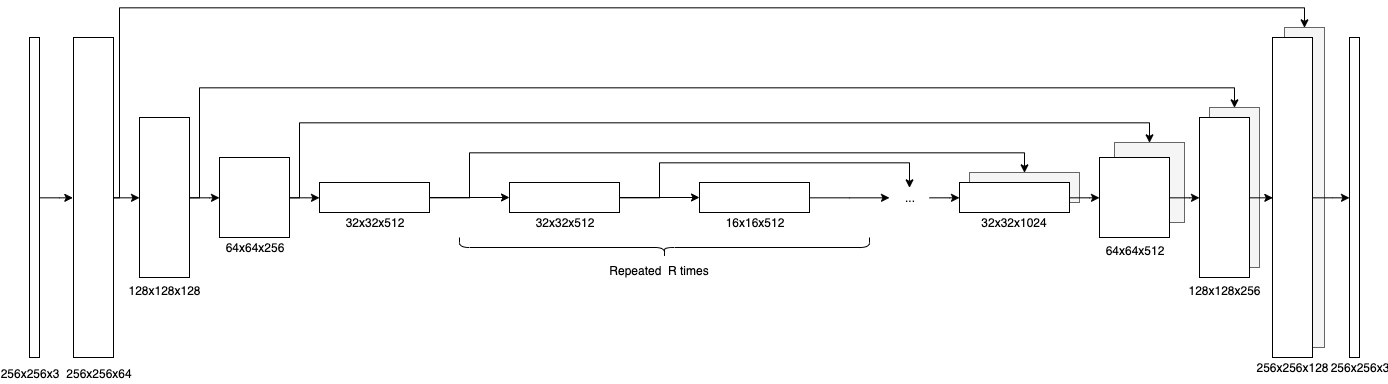
\includegraphics[width=0.9\textwidth]{unet_stain-nn}
\end{figure}

As a means to obtain low-level information
(location, texture, ...) from the encoder,
the output from the corresponding encoder layer is concatenated to the output
of the previous decoder layer.

\end{frame}

\subsection{Inference technique}

\begin{frame}{Why?}
\begin{block}{Need}
Whole slide images are too large to fit directly on a GPU, therefore,
the inference has to be tile-by-tile to obtain the stain transformed result.
\end{block}\pause

\begin{alertblock}{Problem}
This introduces artifacts between adjacent tiles in the output due to
instance normalization relying on tile statistics.
\end{alertblock}

\begin{figure}
\centering
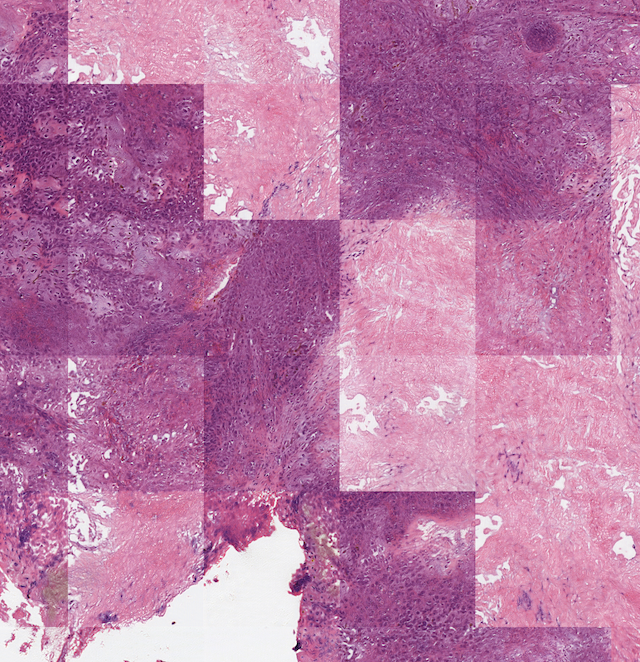
\includegraphics[width=0.3\linewidth]{tiling-example}
\end{figure}

\end{frame}

\begin{frame}{Method I}
\begin{figure}
\centering
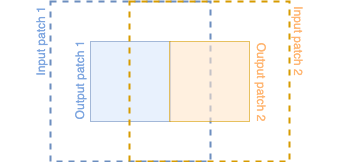
\includegraphics[width=0.3\linewidth]{no-overlap}
\caption{The tiles predictions share context but the outputs do not overlap.}
\end{figure}
\end{frame}

\begin{frame}{Method I - Example}

\begin{columns}

\begin{column}{0.5\textwidth}
\begin{figure}
\centering
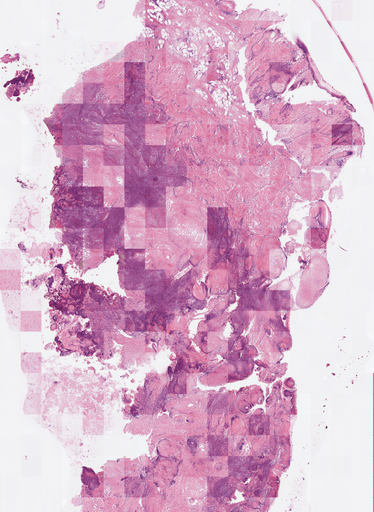
\includegraphics[width=0.75\linewidth]{scan6-independent}
\caption{Independent tile-by-tile inference}
\end{figure}
\end{column}

\begin{column}{0.5\textwidth}
\begin{figure}
\centering
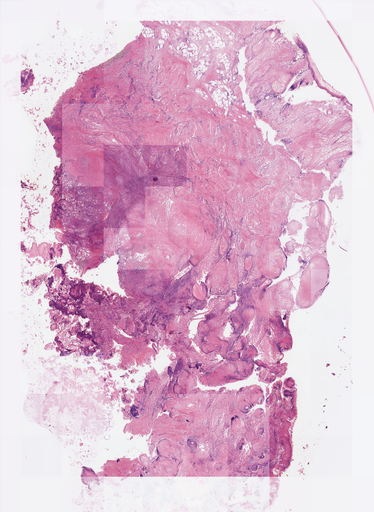
\includegraphics[width=0.75\linewidth]{scan6-no-overlap}
\caption{Tile-by-tile inference using method I}
\end{figure}
\end{column}

\end{columns}

\end{frame}

\begin{frame}{Method II}

\begin{columns}

\begin{column}{0.5\textwidth}
\begin{figure}
\centering
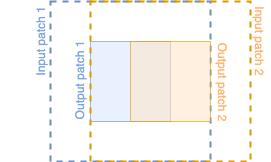
\includegraphics[width=0.8\linewidth]{pyramid}
\caption{Shifting the window by quarter of its size creates an overlap between
the tiles output.}
\end{figure}\pause
\end{column}

\begin{column}{0.5\textwidth}
\begin{figure}
\centering
\includegraphics[width=0.7\linewidth]{weights}
\caption{Output is weighted by a ``pyramidal'' window.
Therefore, each pixel value in the final transformation is a weighted sum of 4 predictions.}
\end{figure}
\end{column}

\end{columns}

\end{frame}

\begin{frame}{Method II - Example}

\begin{columns}

\begin{column}{0.5\textwidth}
\begin{figure}
\centering
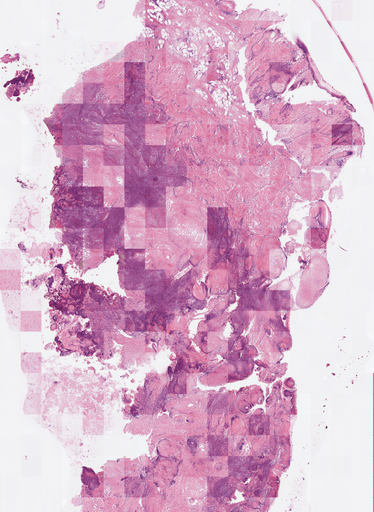
\includegraphics[width=0.75\linewidth]{scan6-independent}
\caption{Independent tile-by-tile inference}
\end{figure}
\end{column}

\begin{column}{0.5\textwidth}
\begin{figure}
\centering
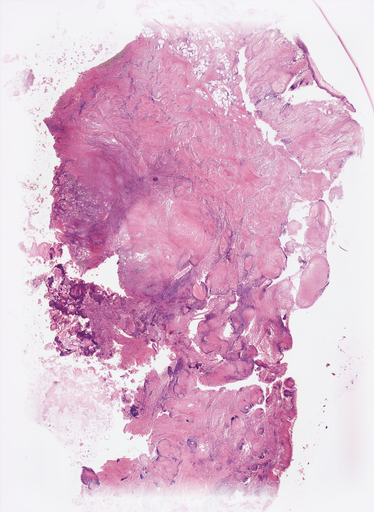
\includegraphics[width=0.75\linewidth]{scan6-pyramid}
\caption{Tile-by-tile inference using method II}
\end{figure}
\end{column}

\end{columns}

\end{frame}

\subsection{Quality measure}

\begin{frame}{Hallucinations}
Two metrics are used to try to measure if the generated
samples contain structures that are not present in the source image
(popularly known as hallucinations). The metrics are based on comparing
the generated image with the equivalent linear staining image (both in gray-scale).

\begin{figure}
\centering
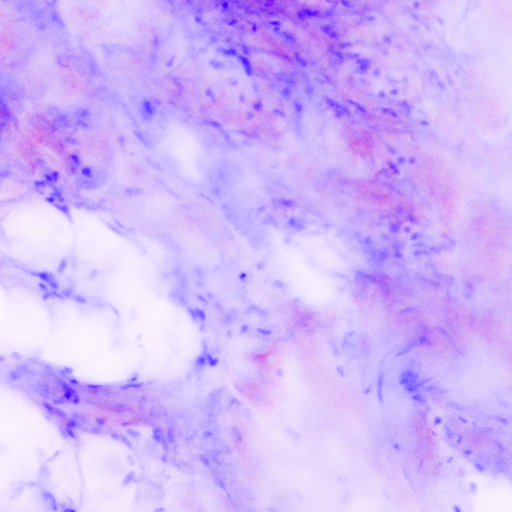
\includegraphics[width=0.3\textwidth]{epoch246_real_A}\hspace{0.15\textwidth}%
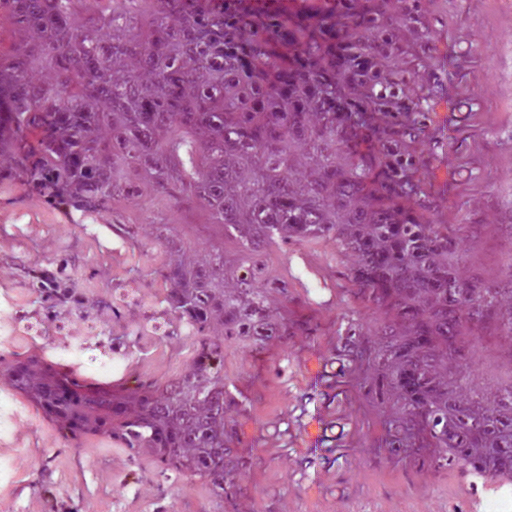
\includegraphics[width=0.3\textwidth]{epoch246_fake_B}
\caption{An example of an hallucination}
\end{figure}

\end{frame}

\begin{frame}{Metrics}

\begin{columns}

\begin{column}{0.5\textwidth}
\begin{block}{SSIM}
To validate the structure integrity of the transformed wholeslides, the
SSIM metric is used.
SSIM is a perception-based model that considers image degradation as
perceived change in structural information.
\end{block}
\end{column}

\begin{column}{0.5\textwidth}

\begin{block}{LBP histogram distance}
Use the Local Binary Patterns (LBP) descriptor to measure the distance
in a texture sense.
\end{block}

\begin{figure}
\centering
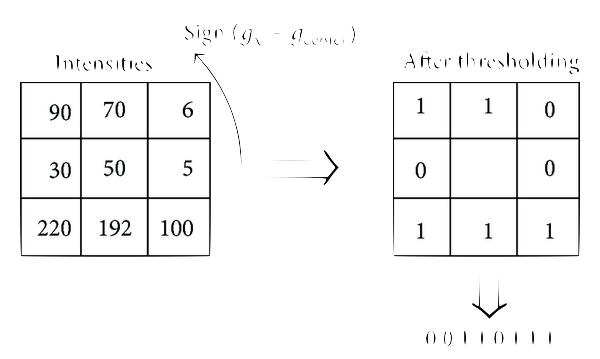
\includegraphics[width=0.7\textwidth]{lbp}
\caption{The distance between the result and source is measured using
the chi-squared distance between the normalized LBP histograms}
\end{figure}

\end{column}

\end{columns}

\end{frame}


\section{Results}

\subsection{Despeckling}

\begin{frame}{Quantitative results}

\begin{table}
\centering
\begin{tabular}{*5c}
\toprule
Model & $M$ & $K$ & $N$ & mean $SSIM$ \\
\midrule
Multiply ($L = 1$) & 3 & 32 & 5 & 0.877 \\
Multiply ($L = 1$) & 5 & 64 & 5 & 0.728 \\
Multiply ($L = 5$) & 3 & 32 & 5 & 0.960 \\
Multiply ($L = 5$) & 5 & 64 & 5 & 0.947 \\

Log-Add ($L = 1$) & 3 & 32 & 5 & 0.960 \\
Log-Add ($L = 1$) & 5 & 64 & 5 & 0.806 \\
Log-Add ($L = 5$) & 3 & 32 & 5 & 0.968 \\
Log-Add ($L = 5$) & 5 & 64 & 5 & 0.965 \\
\bottomrule
\end{tabular}
\caption{Models comparison with different number of layers $M$, number
of filters $K$ and filter size $N$. The validation set mean $SSIM_{input}$
is 0.414 for $L=1$ and 0.723 for $L=5$.}
\end{table}

\end{frame}

\begin{frame}{Qualitative results}

Good SSIM is obtained when comparing a noise-free FCM and its denoised version;
but when applying the DespeckleNN to RCM images,
the result looks noisier.

\begin{figure}
\centering
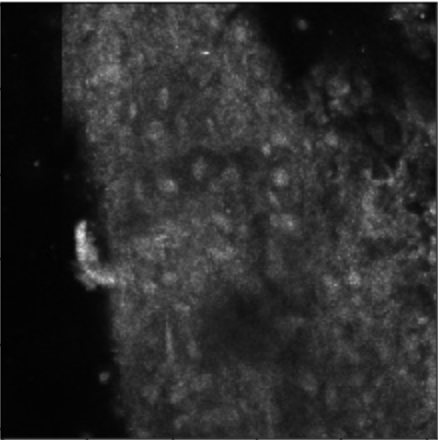
\includegraphics[width=.3\linewidth]{noisy-R}\hspace{0.15\textwidth}%
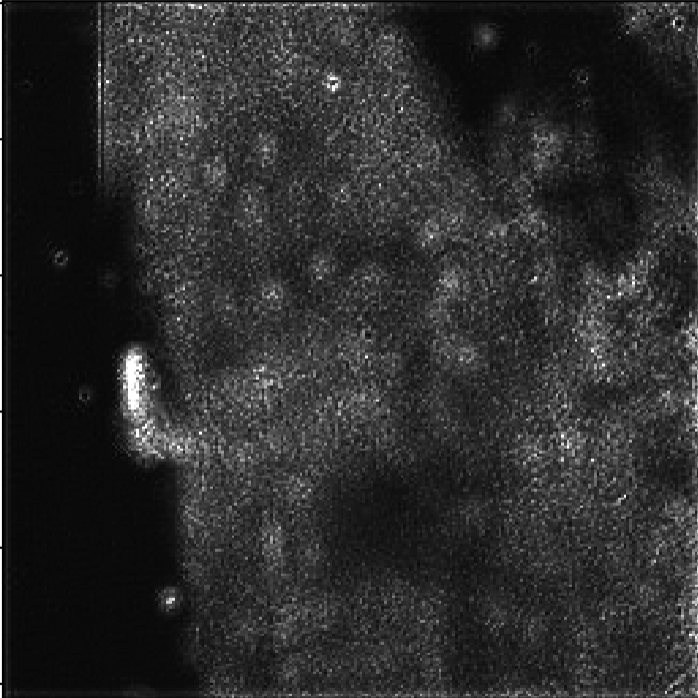
\includegraphics[width=.3\linewidth]{denoised-R}
\end{figure}

\end{frame}

\subsection{Stain}

% TODO Ejemplos de transformacion a lo largo del entrenamiento

\begin{frame}{Quantitative results}
\begin{table}
\centering
\begin{tabular}{l|cc}
\toprule
Metric & Residual & UNet-like \\
\midrule
LBP histogram chi-squared distance & 0.0332 & 0.0183 \\
SSIM & 0.5002 & 0.5570 \\
\bottomrule
\end{tabular}
\caption{Metrics mean values on validation set for the two tested models.}
\label{tab:validation-stain}
\end{table}
\end{frame}

\begin{frame}{Qualitative results}

\begin{columns}

\begin{column}{0.6\textwidth}
\begin{figure}
\centering
\includegraphics[scale=0.3]{104_real_A}\\
\vfill
\includegraphics[scale=0.3]{104_fake_B-resnet}\hspace{0.15\textwidth}%
\includegraphics[scale=0.3]{104_fake_B-unet}
\caption{(N) Linear stain (SW) Residual model stain (SE) Unet model stain}
\end{figure}
\end{column}

\begin{column}{0.4\textwidth}
The motivation behind using the UNet-like model is to mantain the structure,
in practice this generally holds but still some structures
are ``hallucinated'' and nuclei present in the source image are eliminated
(evaluation supported by dermatology expert).
\end{column}

\end{columns}

\end{frame}

\subsection{Inference technique}

\begin{frame}{Experiments}
\begin{figure}
\centering
     \only<1>{
     \includegraphics[width=0.8\textwidth]{inference-experiment-1}
     \caption{7 whole slides are used to compute the metrics}
     }
     \only<2>{
     \includegraphics[width=0.8\textwidth]{inference-experiment-2}
     \caption{The corresponding linear stain and StainNN transformations (with different inference methods) are applied}
     }
     \only<3>{
     \includegraphics[width=0.8\textwidth]{inference-experiment-3}
     \caption{The metrics between the StainNN and linear versions are computed in 500x500 patches}
     }
\end{figure}

\end{frame}

\begin{frame}{SSIM}
\begin{figure}
\centering
\includegraphics[width=0.65\linewidth]{inference-boxplot-ssim}
\caption{The pyramid
tiling (method II) distributions in particular has a higher variability compared to the
other ones, but the general ditribution is always higher.}
\end{figure}
\end{frame}

\begin{frame}{LBP}
\begin{figure}
\centering
\includegraphics[width=0.65\linewidth]{inference-boxplot-lbp}
\caption{The distributions for the pyramid (method II) tend to be in a lower range and
have less variability.}
\end{figure}
\end{frame}


\section{Conclusions and future development}

\begin{frame}{Conclusions}
\begin{itemize}
\item The use of the CycleGANs framework for digitally staining CM slides
has been studied, as well as fully-convolutional models for speckle denoising.
\item Different inference techniques for whole slides are developed and compared.
\item A way of measuring StainNN hallucinations is studied.
\item UNet-like architecture is superior to the
residual one based on both the LBP and SSIM metrics, but
still the structures are not always preserved.
\end{itemize}
\end{frame}

\begin{frame}{Future development}
\begin{enumerate}
\item Find a way to train despeckling model that generalizes to RCM.
\item A new stain model
should be trained with a loss that further encourages structure integrity:
\begin{itemize}
\item Showing both the input and output to the discriminator.
\item Modify the CycleGAN loss.
\end{itemize}
\end{enumerate}
\end{frame}

\end{document}
